\documentclass[12pt]{beamer}
\usepackage{../Estilos/BeamerMAF}
\usepackage{../Estilos/ColoresLatex}
\usepackage{media9}
\usetheme{Warsaw}
\usecolortheme{seahorse}
%\useoutertheme{default}
\setbeamercovered{invisible}
% or whatever (possibly just delete it)
\setbeamertemplate{section in toc}[sections numbered]
\setbeamertemplate{subsection in toc}[subsections numbered]
\setbeamertemplate{subsection in toc}{\leavevmode\leftskip=3.2em\rlap{\hskip-2em\inserttocsectionnumber.\inserttocsubsectionnumber}\inserttocsubsection\par}
\setbeamercolor{section in toc}{fg=blue}
\setbeamercolor{subsection in toc}{fg=blue}
\setbeamercolor{frametitle}{fg=blue}
\setbeamertemplate{caption}[numbered]

\setbeamertemplate{footline}
\beamertemplatenavigationsymbolsempty
\setbeamertemplate{headline}{}


\makeatletter
\setbeamercolor{section in foot}{bg=gray!30, fg=black!90!orange}
\setbeamercolor{subsection in foot}{bg=blue!30}
\setbeamercolor{date in foot}{bg=black}
\setbeamertemplate{footline}
{
  \leavevmode%
  \hbox{%
  \begin{beamercolorbox}[wd=.333333\paperwidth,ht=2.25ex,dp=1ex,center]{section in foot}%
    \usebeamerfont{section in foot} \insertsection
  \end{beamercolorbox}%
  \begin{beamercolorbox}[wd=.333333\paperwidth,ht=2.25ex,dp=1ex,center]{subsection in foot}%
    \usebeamerfont{subsection in foot}  \insertsubsection
  \end{beamercolorbox}%
  \begin{beamercolorbox}[wd=.333333\paperwidth,ht=2.25ex,dp=1ex,right]{date in head/foot}%
    \usebeamerfont{date in head/foot} \insertshortdate{} \hspace*{2em}
    \insertframenumber{} / \inserttotalframenumber \hspace*{2ex} 
  \end{beamercolorbox}}%
  \vskip0pt%
}
\makeatother

\makeatletter
\patchcmd{\beamer@sectionintoc}{\vskip1.5em}{\vskip0.8em}{}{}
\makeatother

\newlength{\depthofsumsign}
\setlength{\depthofsumsign}{\depthof{$\sum$}}
\newcommand{\nsum}[1][1.4]{% only for \displaystyle
    \mathop{%
        \raisebox
            {-#1\depthofsumsign+1\depthofsumsign}
            {\scalebox
                {#1}
                {$\displaystyle\sum$}%
            }
    }
}
\def\scaleint#1{\vcenter{\hbox{\scaleto[3ex]{\displaystyle\int}{#1}}}}
\def\scaleoint#1{\vcenter{\hbox{\scaleto[3ex]{\displaystyle\oint}{#1}}}}
\def\bs{\mkern-12mu}


\AtBeginDocument{\RenewCommandCopy\qty\SI}
\ExplSyntaxOn
\msg_redirect_name:nnn { siunitx } { physics-pkg } { none }
\ExplSyntaxOff

\makeatletter
% \setbeamercolor{section in foot}{bg=gray!30, fg=black!90!orange}
% \setbeamercolor{subsection in foot}{bg=blue!30!yellow, fg=red}
% \setbeamercolor{date in foot}{bg=black, fg=white}
\setbeamertemplate{footline}
{
  \leavevmode%
  \hbox{%
  \begin{beamercolorbox}[wd=.333333\paperwidth,ht=2.25ex,dp=1ex,center]{section in foot}%
    \usebeamerfont{section in foot} \insertsection
  \end{beamercolorbox}%
  \begin{beamercolorbox}[wd=.333333\paperwidth,ht=2.25ex,dp=1ex,center]{subsection in foot}%
    \usebeamerfont{subsection in foot}  \insertsubsection
  \end{beamercolorbox}%
  \begin{beamercolorbox}[wd=.333333\paperwidth,ht=2.25ex,dp=1ex,right]{date in head/foot}%
    \usebeamerfont{date in head/foot} \insertshortdate{} \hspace*{2em}
    \insertframenumber{} / \inserttotalframenumber \hspace*{2ex} 
  \end{beamercolorbox}}%
  \vskip0pt%.0
}
\makeatother

\newcommand{\includemovie}[3]{%
\includemedia[
  width=0.8\linewidth, % ancho del video
  height=0.6\linewidth, % alto del video
  activate=onclick,     % se reproduce al hacer clic
  addresource=membrana_03.mp4,% archivo de video
  flashvars={
     source=membrana_03.mp4   % ruta del video
    &autoPlay=true      % reproducción automática (opcional)
  }%
]{}{StrobeMediaPlayback.swf}%
}% end of the new command

\date{14 de agosto de 2025}

\title{La física y la geometría}
\subtitle{Objetivos del Tema 1}

\begin{document}

\maketitle
\fontsize{14}{14}\selectfont
\spanishdecimal{.}

\section*{Contenido}
\frame[allowframebreaks]{\frametitle{Contenido} \tableofcontents[currentsection, hideallsubsections]}

\section{Introducción}
\frame[allowframebreaks]{\frametitle{Temas a revisar} \tableofcontents[currentsection, hideothersubsections]}
\subsection{Sistemas conocidos}

\begin{frame}
\frametitle{Introducción}
Estamos familiarizados con el uso de distintos sistemas coordenados para describir problemas físicos.
\\
\bigskip
\pause
Hemos usado coordenadas cartesianas, cilíndricas y esféricas para problemas con esas simetrías.
\end{frame}
\begin{frame}
\frametitle{Otros sistemas}
Veremos que existen otros sistemas coordenados que poco a poco durante la carrera, nos encontraremos con ellos para problemas en particular.
\\
\bigskip
\pause
El Tema 1 nos brindará una estrategia de trabajo con ellos.
\end{frame}

% \section{Ejemplos}
% \frame{\tableofcontents[currentsection, hideothersubsections]}
% \subsection{Dos ejemplos}

\begin{frame}
\frametitle{Primer ejemplo}
Consideremos el vector campo eléctrico $(\va{E})$ creado por una carga puntual $q$ localizada en el origen de un sistema cartesiano.
\end{frame}
\begin{frame}
\frametitle{Primer ejemplo}
Usando los vectores de la base canónica en $\mathbb{R}^{3}$
\begin{figure}[H]
  \centering
  \includegraphics[scale=1]{Imagenes/objetivos_01.pdf}
\end{figure}
\end{frame}
\begin{frame}
\frametitle{Primer ejemplo}
El campo eléctrico es:
\pause
\begin{align*}
\va{E} = \dfrac{q}{4 \pi \varepsilon_{0}} \, \dfrac{x \, \vu{e}_{x} + y \, \vu{e}_{y} + z \, \vu{e}_{z}}{\left( x^{2} + y^{2} + z^{2} \right)^{3/2}}
\end{align*}
\end{frame}
\begin{frame}
\frametitle{Primer ejemplo}
En coordenadas esféricas $(r, \varphi, \theta)$, en donde se aprovecha completamente la simetría del problema para este campo:
\begin{figure}[H]
  \centering
  \includegraphics[scale=0.8]{Imagenes/objetivos_02.pdf}
\end{figure}
\end{frame}
\begin{frame}
\frametitle{Primer ejemplo}
La expresión anterior se simplifica, \pause así el campo eléctrico resulta ser:
\begin{align*}
\va{\vb{E}} = \dfrac{q}{4 \pi \varepsilon_{0}} \, \dfrac{\vu{e}_{r}}{r^{2}}
\end{align*}
\end{frame}
\begin{frame}
\frametitle{¿Cómo cambiamos de un sistema a otro?}
Será necesario utilizar conceptos como:
\pause
\setbeamercolor{item projected}{bg=bananayellow,fg=black}
\setbeamertemplate{enumerate items}{%
\usebeamercolor[bg]{item projected}%
\raisebox{1.5pt}{\colorbox{bg}{\color{fg}\footnotesize\insertenumlabel}}%
}
\begin{enumerate}[<+->]
\item Reglas de transformación.
\item Factores de escala.
\item Vectores base unitarios.
\end{enumerate}
\end{frame}
\begin{frame}
\frametitle{Operadores diferenciales necesarios}
Posteriormente tendremos que representar en el nuevo sistema coordenado, al conjunto de operadores diferenciales que ya conocemos:
\pause
\setbeamercolor{item projected}{bg=corn,fg=cordovan}
\setbeamertemplate{enumerate items}{%
\usebeamercolor[bg]{item projected}%
\raisebox{1.5pt}{\colorbox{bg}{\color{fg}\footnotesize\insertenumlabel}}%
}
\begin{enumerate}[<+->]
\item Gradiente.
\item Divergencia.
\item Rotacional.
\item Laplaciano.
\end{enumerate}
\end{frame}
\begin{frame}
\frametitle{Segundo ejemplo}
Ahora consideramos un problema con ondas estacionarias en un sistema bidimensional con simetría circular: \pause una membrana circular delgada y perfectamente flexible.
\end{frame}
\begin{frame}
\frametitle{Segundo ejemplo}
Por ejemplo: una membrana idealizada de tambor circular de radio $r$.
\begin{figure}[H]
  \centering
  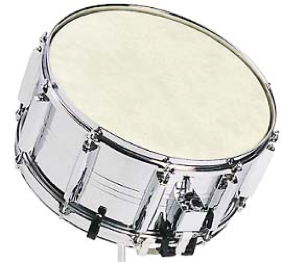
\includegraphics[scale=0.75]{Imagenes/Tambor.png}
\end{figure}
\end{frame}
\begin{frame}
\frametitle{Segundo ejemplo}
La ecuación de onda en coordenadas bidimensionales cilíndricas $(x , y \rightarrow r, \varphi)$ para la amplitud de desplazamiento, $\psi (r, \varphi, t)$ viene dada por:
\pause
\begin{align*}
\laplacian \psi (r, \varphi, t) - \dfrac{1}{v^{2}} \pdv[2]{\psi (r, \varphi, t)}{t} = 0
\end{align*}
\end{frame}
\begin{frame}
\frametitle{Elegir el sistema coordenado}
Para la elección del sistema coordenado debemos de considerar aquel en donde la simetría del problema nos simplique el trabajo.
\\
\bigskip
\pause
En este caso, corresponde elegir el sistema coordenado cilíndrico.
\end{frame}
\begin{frame}
\frametitle{Geometría del sistema cilíndrico}
\begin{figure}[H]
  \centering
  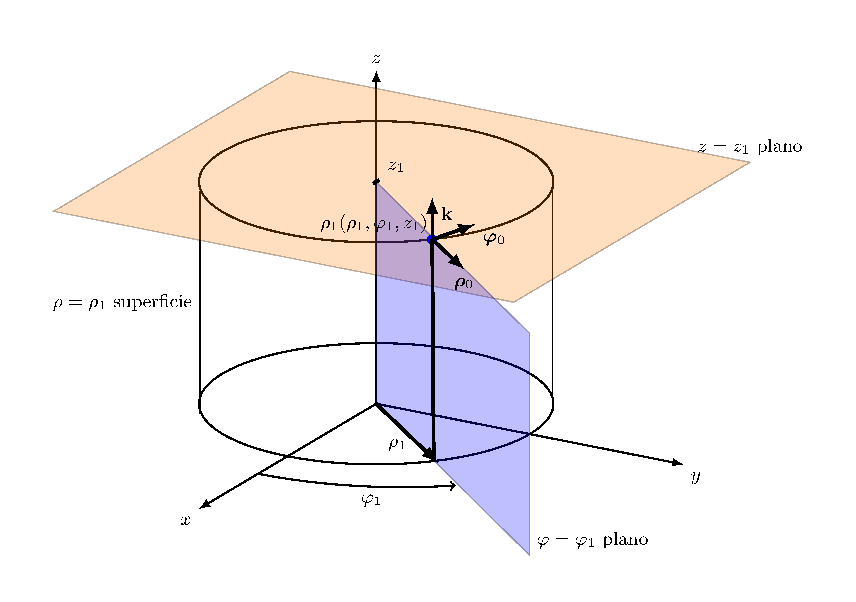
\includegraphics[scale=0.7]{Imagenes/Coordenadas_Cilindricas_01.eps}
\end{figure}
\end{frame}
\begin{frame}
\frametitle{Reexpresar la ecuación de onda}
Una vez elegido el sistema coordenado, debemos de realizar lo necesario para reexpresar la ecuación diferencial del problema en el sistema.
\\
\bigskip
\pause
Habrá que \enquote{adaptar} el operador Laplaciano en este sistema.
\end{frame}
\begin{frame}
\frametitle{Solución a la ED obtenida}
Una vez que se realiza la reexpresión de la ED, el siguiente paso es resolverla.
\\
\bigskip
\pause
Para ello, ocuparemos lo que se revisará en el \emph{\textocolor{blue}{Tema 2 - Primeras técnicas de solución}}.
\end{frame}
\begin{frame}
\frametitle{Solución al problema}
Cuando veamos el tema de \textocolor{darkgreen}{función de Bessel}, tomaremos de nuevo este ejercicio.
\\
\bigskip
\pause
La solución obtenida la podemos ocupar con otras herramientas computacionales para \emph{simular} el comportamiento de la membrana circular.
\end{frame}
\begin{frame}
\frametitle{Simulación computacional}
\begin{figure}[h!]
    \centering
    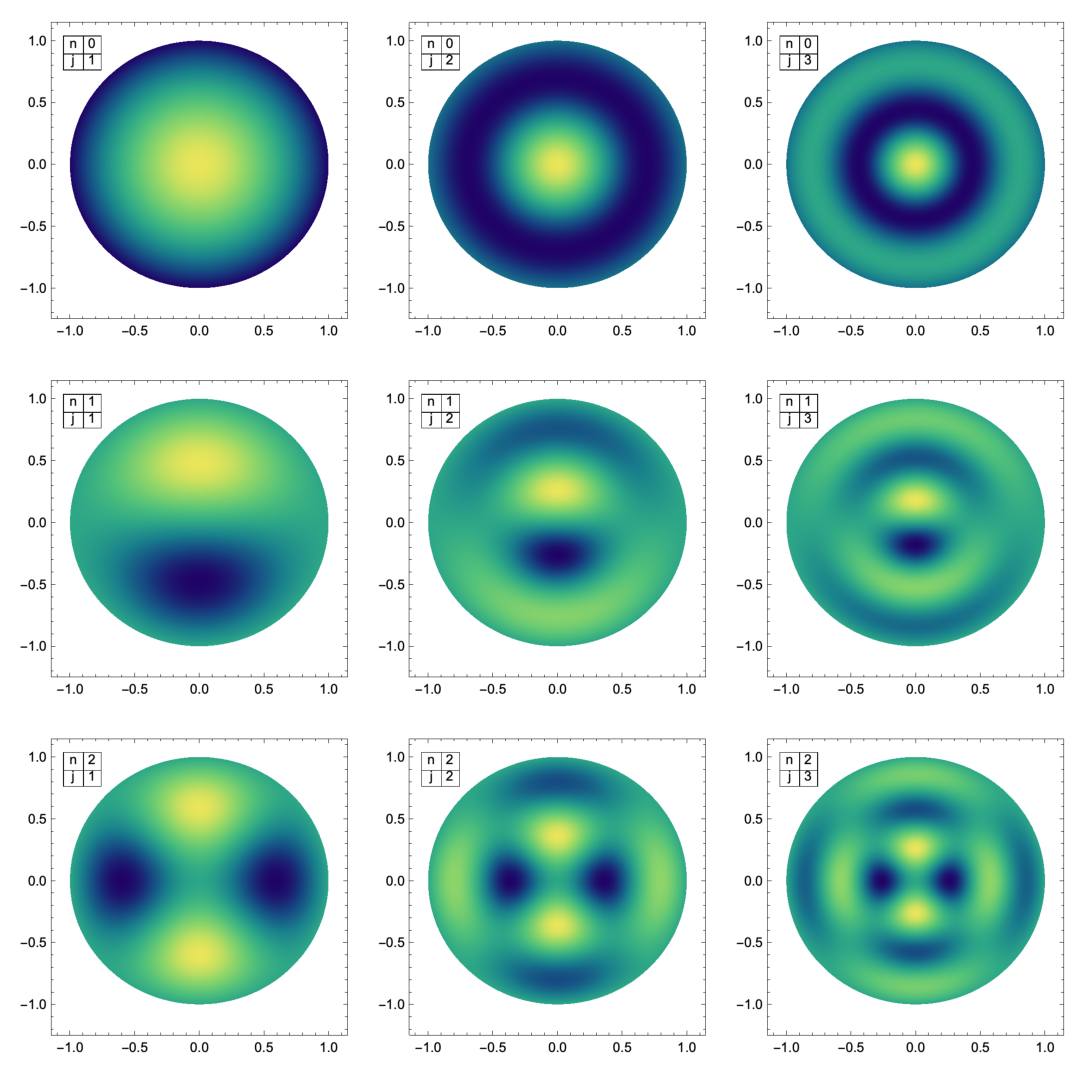
\includegraphics[scale=0.32]{Imagenes/Modos_Vibracion_Membrana_Circular_01.eps}
\end{figure}
\end{frame}
\begin{frame}
\frametitle{Simulación computacional - Video}
% \movie[
%   width=0.8\linewidth,
%   height=0.6\linewidth,
%   poster,   % muestra la primera imagen (poster frame)
%   autostart % opcional, depende del visor
% ]{\fbox{Reproducir video}}{membrana_03.mp4}
% \begin{center}%
%     \includemovie{.85\textheight}{.85\textheight}{membrana_03.mp4}%
% \end{center}
 \centering
    \movie[externalviewer]{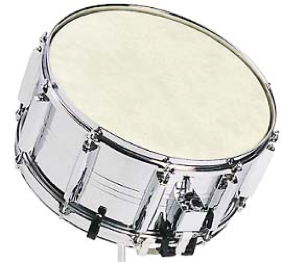
\includegraphics[width=0.5\textheight, keepaspectratio]{Imagenes/Tambor.png}}{membrana_03.mp4}
\end{frame}
\begin{frame}
\frametitle{¿Y si tenemos un toroide?}
\begin{figure}
   \centering
    \movie[externalviewer]{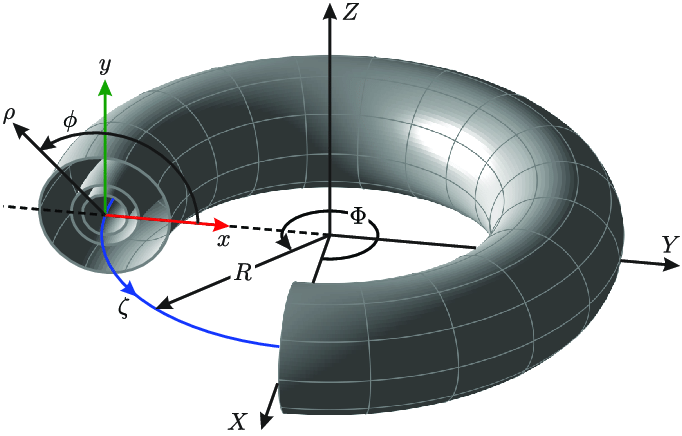
\includegraphics[width=\textheight, keepaspectratio]{Imagenes/Geometria_Toro.png}}{Toroide.mp4}  
  
  % \centering
  %   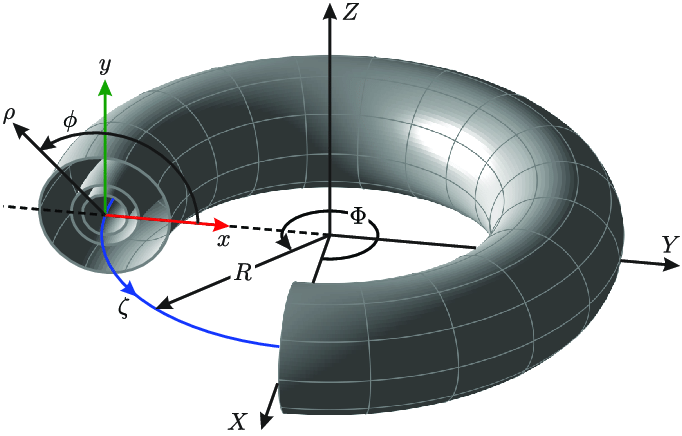
\includegraphics[scale=0.4]{Imagenes/Geometria_Toro.png}
\end{figure}
\end{frame}

\section{Sistemas coordenados}
\frame{\frametitle{Temas a revisar} \tableofcontents[currentsection, hideothersubsections]}
\subsection{Sistemas comunes}

\begin{frame}
\frametitle{Sistemas coordenados más comunes}
A continuación se enlistarán una serie de sistemas coordenados que serán muy comunes de encontrar en la física, siendo muy específicos para un problema determinado.
\end{frame}
\begin{frame}
\frametitle{Aviso importante}
Se menciona oportunamente que \textocolor{red}{no se revisarán todos} en este primer tema.
\\
\bigskip
\pause
Aprenderemos la base de trabajo para analizar otro sistema que se nos presente en un futuro.
\end{frame}
\begin{frame}
\frametitle{Sistemas coordenados}
\setbeamercolor{item projected}{bg=darkorange,fg=black}
\setbeamertemplate{enumerate items}{%
\usebeamercolor[bg]{item projected}%
\raisebox{1.5pt}{\colorbox{bg}{\color{fg}\footnotesize\insertenumlabel}}%
}
\begin{enumerate}[<+->]
\item Cartesiano.
\item Esféricas polares.
\item Cilíndricas polares.
\item Cilíndricas parabólicas.
\item Cilíndricas elípticas.
\item Cilíndricas bipolares.
\item Esferoidales prolatas.
\item Esferoidales oblatas.
\seti
\end{enumerate}
\end{frame}
\begin{frame}
\frametitle{Sistemas coordenados}
\setbeamercolor{item projected}{bg=darkorange,fg=black}
\setbeamertemplate{enumerate items}{%
\usebeamercolor[bg]{item projected}%
\raisebox{1.5pt}{\colorbox{bg}{\color{fg}\footnotesize\insertenumlabel}}%
}\begin{enumerate}[<+->]
\conti
\item Parabólicas.
\item Elipsoidal.
\item Toroidal.
\item Biesféricas.
\item Cónicas.
\item Elipsoidales confocales.
\item Parabólicas confocales.
\end{enumerate}
\end{frame}
\begin{frame}
\frametitle{Otros sistemas coordenados}
Cuando se realizan ciertas traslaciones en alguna dirección perpendicular en particular de los sistemas mencionados, o cuando se tienen superficies coordenadas que son planos paralelos, \pause se obtiene un conjunto particular de sistemas coordenados.
\end{frame}
\begin{frame}
\frametitle{Sistemas coordenados especiales}
\setbeamercolor{item projected}{bg=debianred,fg=white}
\setbeamertemplate{enumerate items}{%
\usebeamercolor[bg]{item projected}%
\raisebox{1.5pt}{\colorbox{bg}{\color{fg}\footnotesize\insertenumlabel}}%
}
\begin{enumerate}[<+->]
\item Cilíndrico tangente.
\item Cilíndrico cardioide.
\item Cilíndrico hiperbólico.
\item Cilíndrico logarítmico.
\item Coordenadas Zeta.
\end{enumerate}
\end{frame}

\section{Ecs. Física Matemática}
\frame{\frametitle{Temas a revisar} \tableofcontents[currentsection, hideothersubsections]}
\subsection{La ecuación de Helmholtz}

\begin{frame}
\frametitle{La ecuación de Helmholtz}
La ecuación de Helmholtz se encuentra muy a menudo en la física:
\pause
\begin{align*}
\laplacian{\psi} + k^{2} \, \psi = 0
\end{align*}
\end{frame}
\begin{frame}
\frametitle{¿De dónde surge la ecuación de Helmholtz?}
La ecuación de Helmholtz la podemos interpretar \enquote{como un puente} entre la ecuación de onda y los problemas estacionarios que aparecen en muchas ramas de la física.
\end{frame}
\begin{frame}
\frametitle{La ecuación de Helmholtz}
Ejemplos en donde encontraremos esta ecuación:
\pause
\setbeamercolor{item projected}{bg=bubbles,fg=burgundy}
\setbeamertemplate{enumerate items}{%
\usebeamercolor[bg]{item projected}%
\raisebox{1.5pt}{\colorbox{bg}{\color{fg}\footnotesize\insertenumlabel}}%
}
\begin{enumerate}[<+->]
\item Acústica: presión sonora en una cavidad (modos propios).
\item Electromagnetismo: modos de una guía de ondas o cavidad resonante.
\item Óptica: propagación de luz en medios homogéneos.
\seti
\end{enumerate}
\end{frame}
\begin{frame}
\frametitle{La ecuación de Helmholtz}
\setbeamercolor{item projected}{bg=bubbles,fg=burgundy}
\setbeamertemplate{enumerate items}{%
\usebeamercolor[bg]{item projected}%
\raisebox{1.5pt}{\colorbox{bg}{\color{fg}\footnotesize\insertenumlabel}}%
}
\begin{enumerate}[<+->]
\conti
\item Mecánica cuántica: partícula libre o en pozo de potencial con energía fija (la ecuación de Schrödinger estacionaria es una de Helmholtz con $k^{2} \propto E$)
\item Vibraciones mecánicas: modos propios de una membrana, cuerda o placa.
\end{enumerate}
\end{frame}
\begin{frame}
\frametitle{La ecuación de Helmholtz}
En la ecuación de Schrödinger dependiente del tiempo es:
\pause
\begin{align*}
i \, \hbar \, \pdv{\Psi}{t} = \left[ - \dfrac{\hbar^{2}}{2 \, m} \, \laplacian{\phi} + V (\vb{r}) \right] \, \Psi
\end{align*}
\end{frame}
\begin{frame}
\frametitle{La ecuación de Helmholtz}
Si consideramos una solución de la forma:
\begin{align*}
\Psi (\vb{r}, t) = \psi (\vb{r}) \, e^{- i \, E \, t / \hbar} 
\end{align*}
\pause
La ecuación inicial es:
\begin{align*}
E \, \psi = \left( - \dfrac{\hbar^{2}}{2 m} \, \laplacian + V \right) \, \psi
\end{align*}
\end{frame}
\begin{frame}
\frametitle{La ecuación de Helmholtz}
Entonces:
\pause
\begin{align*}
\laplacian \psi + \dfrac{2 m}{\hbar^{2}} \, (E - V) \, \psi = 0
\end{align*}
\pause
Esto es la ec. de Helmholtz con índice espacial:
\begin{align*}
  \left[ \laplacian + k^{2} (\vb{r}) \right] \, \psi = 0, \hspace{1cm} k^{2} (\vb{r}) = \dfrac{2 m}{\hbar^{2}} \, (E - V (\vb{r}))
\end{align*}
\end{frame}
\begin{frame}
\frametitle{La ecuación de Helmholtz}
Un buen ejercicio que nos brindará el desarrollo de habilidades trabajando con distintos sistemas coordenados, es expresar esta ecuación diferencial en cada uno de los sistemas coordenados que hemos mencionado.
\end{frame}
\begin{frame}
\frametitle{La ecuación de Helmholtz}
Con lo que veremos en el Tema 1 y al inicio del Tema 2, encontramos que la ecuación es \textocolor{carmine}{separable} en 11 de los sistemas coordenados mencionados previamente.
\end{frame}
\begin{frame}
\frametitle{La ecuación de Helmholtz}
Obtendremos entonces un sistema de ecuaciones diferenciales las cuales se podrán resolver \textocolor{coolblack}{más fácilmente} que en el sistema inicial.
\end{frame}

\subsection{Ecuaciones lineales y no lineales}

\begin{frame}
\frametitle{Otras ecuaciones relevantes en la física}
Enumeremos algunas EDP conocidas:
\pause
\setbeamercolor{item projected}{bg=indigo(web),fg=white}
\setbeamertemplate{enumerate items}{%
\usebeamercolor[bg]{item projected}%
\raisebox{1.5pt}{\colorbox{bg}{\color{fg}\footnotesize\insertenumlabel}}%
}
\begin{enumerate}[<+->]
\item La ecuación de calor:
\begin{align*}
\text{\Large{$u_{t} - u_{xx} = 0$}} \hspace{2cm} \pdv{u}{t} - \pdv[2]{u}{x} = 0
\end{align*}
\item La ecuación de onda:
\begin{align*}
\text{\Large{$u_{tt} - u_{xx} = 0$}}
\end{align*}
\item Ecuación de Laplace:
\begin{align*}
\text{\Large{$u_{xx} + u_{yy} = 0$}}
\end{align*}
\seti
\end{enumerate}
\end{frame}
\begin{frame}
\frametitle{Otras ecuaciones relevantes en la física}
\setbeamercolor{item projected}{bg=indigo(web),fg=white}
\setbeamertemplate{enumerate items}{%
\usebeamercolor[bg]{item projected}%
\raisebox{1.5pt}{\colorbox{bg}{\color{fg}\footnotesize\insertenumlabel}}%
}
\begin{enumerate}[<+->]
\conti
\item Ecuación no lineal de calor:
\begin{align*}
\pdv{u}{t} = \pdv{x} \left[ f(u) \, \pdv{u}{x} \right]
\end{align*}
\seti
\end{enumerate}
\end{frame}
\begin{frame}
\frametitle{Otras ecuaciones relevantes en la física}
\setbeamercolor{item projected}{bg=indigo(web),fg=white}
\setbeamertemplate{enumerate items}{%
\usebeamercolor[bg]{item projected}%
\raisebox{1.5pt}{\colorbox{bg}{\color{fg}\footnotesize\insertenumlabel}}%
}
\begin{enumerate}[<+->]
\conti
\item Ecuación Kolmogorov-Petrovskii-Piskunov:
\begin{align*}
\pdv{u}{t} = a \, \pdv[2]{w}{x} + f(u), \hspace{1cm} a > 0
\end{align*}
\seti
\end{enumerate}
\end{frame}
\begin{frame}
\frametitle{Otras ecuaciones relevantes en la física}
Las ecuaciones de este tipo se encuentran a menudo en varios problemas de transferencia de masa y calor (siendo $f$ la reacción de cambio del volumen en una reacción química), teoría de la combustión, biología y ecología.
\end{frame}
\begin{frame}
\frametitle{Otras ecuaciones relevantes en la física}
\setbeamercolor{item projected}{bg=indigo(web),fg=white}
\setbeamertemplate{enumerate items}{%
\usebeamercolor[bg]{item projected}%
\raisebox{1.5pt}{\colorbox{bg}{\color{fg}\footnotesize\insertenumlabel}}%
}
\begin{enumerate}[<+->]
\conti
\item Ecuación de Burgers:
\begin{align*}
\pdv{w}{t} + u \, \pdv{u}{x} = \pdv[2]{u}{x}
\end{align*}
Se ocupa para describir procesos ondulatorios en la dinámica de gases, hidrodinámica, en acústica y para el flujo del tráfico.
\seti
\end{enumerate}
\end{frame}
\begin{frame}
\frametitle{Otras ecuaciones relevantes en la física}
\setbeamercolor{item projected}{bg=indigo(web),fg=white}
\setbeamertemplate{enumerate items}{%
\usebeamercolor[bg]{item projected}%
\raisebox{1.5pt}{\colorbox{bg}{\color{fg}\footnotesize\insertenumlabel}}%
}
\begin{enumerate}[<+->]
\conti
\item Ecuación de onda no lineal:
\begin{align*}
\pdv[2]{u}{t} = \pdv{x} \left[ f(u) \, \pdv{u}{x} \right]
\end{align*}
Esta ecuación se encuentra en dinámica de ondas y gases, con $f(u) > 0$.
\end{enumerate}
\end{frame}

\section{Objetivos}
\frame{\frametitle{Temas a revisar} \tableofcontents[currentsection, hideothersubsections]}
\subsection{Tema 1}

\begin{frame}
\frametitle{Objetivos}
Al concluir el Tema 1, el alumno:
\pause
\setbeamercolor{item projected}{bg=onyx,fg=white}
\setbeamertemplate{enumerate items}{%
\usebeamercolor[bg]{item projected}%
\raisebox{1.5pt}{\colorbox{bg}{\color{fg}\footnotesize\insertenumlabel}}%
}
\begin{enumerate}[<+->]
\item Describirá las superficies coordenadas a partir de las reglas de transformación entre el sistema cartesiano y otro sistema de estudio.
\seti
\end{enumerate}
\end{frame}
\begin{frame}
\frametitle{Objetivos}
\setbeamercolor{item projected}{bg=onyx,fg=white}
\setbeamertemplate{enumerate items}{%
\usebeamercolor[bg]{item projected}%
\raisebox{1.5pt}{\colorbox{bg}{\color{fg}\footnotesize\insertenumlabel}}%
}
\begin{enumerate}[<+->]
\conti
\item Determinará los factores de escala del nuevo sistema de estudio, así como los vectores base y la interpretación con los vectores cartesianos.
\seti
\end{enumerate}
\end{frame}
\begin{frame}
\frametitle{Objetivos}
\setbeamercolor{item projected}{bg=onyx,fg=white}
\setbeamertemplate{enumerate items}{%
\usebeamercolor[bg]{item projected}%
\raisebox{1.5pt}{\colorbox{bg}{\color{fg}\footnotesize\insertenumlabel}}%
}
\begin{enumerate}[<+->]
\conti
\item Calculará los operadores diferenciales en el nuevo sistema de estudio.
\item Ocupará las funciones Gamma y Beta para resolver ejercicios de la física.
\end{enumerate}
\end{frame}

\section{Materiales complementarios}
\frame{\frametitle{Temas a revisar} \tableofcontents[currentsection, hideothersubsections]}
\subsection{Lecturas recomendadas}

\begin{frame}
\frametitle{Materiales complementarios}
Tendrán disponibles materiales complementarios, que como mencionamos en la presentación del curso, les serán de utilidad ya que cuentan con un enfoque elevado, pero lo necesario para una consulta.
\\
\bigskip
Siendo también un atractivo para que extiendan la consulta en las referencias bibliográficas del curso.
\end{frame}
\begin{frame}
\frametitle{Materiales complementarios}
\begin{figure}
  \centering
  \includegraphics<1>[scale=0.3]{Imagenes/Material_Ley.png}
  \includegraphics<2>[scale=0.25]{Imagenes/Material_Morse.png}
  \includegraphics<3>[scale=0.4]{Imagenes/Material_Nguyen.png}
\end{figure}
\end{frame}

\end{document}